% Options for packages loaded elsewhere
\PassOptionsToPackage{unicode}{hyperref}
\PassOptionsToPackage{hyphens}{url}
\PassOptionsToPackage{dvipsnames,svgnames,x11names}{xcolor}
%
\documentclass[
  letterpaper,
  DIV=11,
  numbers=noendperiod]{scrartcl}

\usepackage{amsmath,amssymb}
\usepackage{iftex}
\ifPDFTeX
  \usepackage[T1]{fontenc}
  \usepackage[utf8]{inputenc}
  \usepackage{textcomp} % provide euro and other symbols
\else % if luatex or xetex
  \usepackage{unicode-math}
  \defaultfontfeatures{Scale=MatchLowercase}
  \defaultfontfeatures[\rmfamily]{Ligatures=TeX,Scale=1}
\fi
\usepackage{lmodern}
\ifPDFTeX\else  
    % xetex/luatex font selection
\fi
% Use upquote if available, for straight quotes in verbatim environments
\IfFileExists{upquote.sty}{\usepackage{upquote}}{}
\IfFileExists{microtype.sty}{% use microtype if available
  \usepackage[]{microtype}
  \UseMicrotypeSet[protrusion]{basicmath} % disable protrusion for tt fonts
}{}
\makeatletter
\@ifundefined{KOMAClassName}{% if non-KOMA class
  \IfFileExists{parskip.sty}{%
    \usepackage{parskip}
  }{% else
    \setlength{\parindent}{0pt}
    \setlength{\parskip}{6pt plus 2pt minus 1pt}}
}{% if KOMA class
  \KOMAoptions{parskip=half}}
\makeatother
\usepackage{xcolor}
\setlength{\emergencystretch}{3em} % prevent overfull lines
\setcounter{secnumdepth}{-\maxdimen} % remove section numbering
% Make \paragraph and \subparagraph free-standing
\makeatletter
\ifx\paragraph\undefined\else
  \let\oldparagraph\paragraph
  \renewcommand{\paragraph}{
    \@ifstar
      \xxxParagraphStar
      \xxxParagraphNoStar
  }
  \newcommand{\xxxParagraphStar}[1]{\oldparagraph*{#1}\mbox{}}
  \newcommand{\xxxParagraphNoStar}[1]{\oldparagraph{#1}\mbox{}}
\fi
\ifx\subparagraph\undefined\else
  \let\oldsubparagraph\subparagraph
  \renewcommand{\subparagraph}{
    \@ifstar
      \xxxSubParagraphStar
      \xxxSubParagraphNoStar
  }
  \newcommand{\xxxSubParagraphStar}[1]{\oldsubparagraph*{#1}\mbox{}}
  \newcommand{\xxxSubParagraphNoStar}[1]{\oldsubparagraph{#1}\mbox{}}
\fi
\makeatother


\providecommand{\tightlist}{%
  \setlength{\itemsep}{0pt}\setlength{\parskip}{0pt}}\usepackage{longtable,booktabs,array}
\usepackage{calc} % for calculating minipage widths
% Correct order of tables after \paragraph or \subparagraph
\usepackage{etoolbox}
\makeatletter
\patchcmd\longtable{\par}{\if@noskipsec\mbox{}\fi\par}{}{}
\makeatother
% Allow footnotes in longtable head/foot
\IfFileExists{footnotehyper.sty}{\usepackage{footnotehyper}}{\usepackage{footnote}}
\makesavenoteenv{longtable}
\usepackage{graphicx}
\makeatletter
\newsavebox\pandoc@box
\newcommand*\pandocbounded[1]{% scales image to fit in text height/width
  \sbox\pandoc@box{#1}%
  \Gscale@div\@tempa{\textheight}{\dimexpr\ht\pandoc@box+\dp\pandoc@box\relax}%
  \Gscale@div\@tempb{\linewidth}{\wd\pandoc@box}%
  \ifdim\@tempb\p@<\@tempa\p@\let\@tempa\@tempb\fi% select the smaller of both
  \ifdim\@tempa\p@<\p@\scalebox{\@tempa}{\usebox\pandoc@box}%
  \else\usebox{\pandoc@box}%
  \fi%
}
% Set default figure placement to htbp
\def\fps@figure{htbp}
\makeatother

\usepackage{booktabs}
\usepackage{longtable}
\usepackage{array}
\usepackage{multirow}
\usepackage{wrapfig}
\usepackage{float}
\usepackage{colortbl}
\usepackage{pdflscape}
\usepackage{tabu}
\usepackage{threeparttable}
\usepackage{threeparttablex}
\usepackage[normalem]{ulem}
\usepackage{makecell}
\usepackage{xcolor}
\KOMAoption{captions}{tableheading}
\makeatletter
\@ifpackageloaded{caption}{}{\usepackage{caption}}
\AtBeginDocument{%
\ifdefined\contentsname
  \renewcommand*\contentsname{Table of contents}
\else
  \newcommand\contentsname{Table of contents}
\fi
\ifdefined\listfigurename
  \renewcommand*\listfigurename{List of Figures}
\else
  \newcommand\listfigurename{List of Figures}
\fi
\ifdefined\listtablename
  \renewcommand*\listtablename{List of Tables}
\else
  \newcommand\listtablename{List of Tables}
\fi
\ifdefined\figurename
  \renewcommand*\figurename{Figure}
\else
  \newcommand\figurename{Figure}
\fi
\ifdefined\tablename
  \renewcommand*\tablename{Table}
\else
  \newcommand\tablename{Table}
\fi
}
\@ifpackageloaded{float}{}{\usepackage{float}}
\floatstyle{ruled}
\@ifundefined{c@chapter}{\newfloat{codelisting}{h}{lop}}{\newfloat{codelisting}{h}{lop}[chapter]}
\floatname{codelisting}{Listing}
\newcommand*\listoflistings{\listof{codelisting}{List of Listings}}
\makeatother
\makeatletter
\usepackage{pdflscape}
\makeatother
\makeatletter
\makeatother
\makeatletter
\@ifpackageloaded{caption}{}{\usepackage{caption}}
\@ifpackageloaded{subcaption}{}{\usepackage{subcaption}}
\makeatother

\usepackage{bookmark}

\IfFileExists{xurl.sty}{\usepackage{xurl}}{} % add URL line breaks if available
\urlstyle{same} % disable monospaced font for URLs
\hypersetup{
  pdftitle={Supplementary},
  colorlinks=true,
  linkcolor={blue},
  filecolor={Maroon},
  citecolor={Blue},
  urlcolor={Blue},
  pdfcreator={LaTeX via pandoc}}


\title{Supplementary}
\author{}
\date{2025-02-26}

\begin{document}
\maketitle


\begin{landscape}

\begin{table}[H]
\centering
\caption{Spatial model summaries for Est  describing effective and nominal dimensions, their ratio, and parameter type across all traits}
\centering
\resizebox{\ifdim\width>\linewidth\linewidth\else\width\fi}{!}{
\fontsize{58}{60}\selectfont
\begin{tabular}[t]{lllllllllllll}
\toprule
\multicolumn{1}{c}{} & \multicolumn{4}{c}{TY} & \multicolumn{4}{c}{TN} & \multicolumn{4}{c}{TV} \\
\cmidrule(l{3pt}r{3pt}){2-5} \cmidrule(l{3pt}r{3pt}){6-9} \cmidrule(l{3pt}r{3pt}){10-13}
  & Effective Dimension & Nominal Dimension & Ratio & Type\textsuperscript{a} & Effective Dimension & Nominal Dimension & Ratio & Type\textsuperscript{a} & Effective Dimension & Nominal Dimension & Ratio & Type\textsuperscript{a}\\
\midrule
Intercept & 1.0 & 1 & 1.00 & F & 1.0 & 1 & 1.00 & F & 1.0 & 1 & 1.00 & F\\
Control & 1.0 & 1 & 1.00 & F & 1.0 & 1 & 1.00 & F & 1.0 & 1 & 1.00 & F\\
Genotype & 505.5 & 604 & 0.84 & R & 483.0 & 604 & 0.80 & R & 539.6 & 604 & 0.89 & R\\
R-Row & 12.2 & 18 & 0.68 & R & 12.2 & 18 & 0.68 & R & 8.5 & 18 & 0.47 & R\\
R-Column & 0.0 & 63 & 0.00 & R & 0.0 & 63 & 0.00 & R & 0.0 & 63 & 0.00 & R\\
\addlinespace
Column & 1.0 & 1 & 1.00 & S & 1.0 & 1 & 1.00 & S & 1.0 & 1 & 1.00 & S\\
Row & 1.0 & 1 & 1.00 & S & 1.0 & 1 & 1.00 & S & 1.0 & 1 & 1.00 & S\\
Column:Row & 1.0 & 1 & 1.00 & S & 1.0 & 1 & 1.00 & S & 1.0 & 1 & 1.00 & S\\
f(Column) & 2.9 & 21 & 0.14 & S & 3.4 & 21 & 0.16 & S & 0.9 & 21 & 0.04 & S\\
f(Row) & 0.0 & 66 & 0.00 & S & 0.0 & 66 & 0.00 & S & 0.0 & 66 & 0.00 & S\\
\addlinespace
f(Column):Row & 3.8 & 21 & 0.18 & S & 0.0 & 21 & 0.00 & S & 3.0 & 21 & 0.14 & S\\
Column:f(Row) & 0.7 & 66 & 0.01 & S & 0.6 & 66 & 0.01 & S & 0.0 & 66 & 0.00 & S\\
f(Column):f(Row) & 16.5 & 1386 & 0.01 & S & 11.7 & 1386 & 0.01 & S & 2.9 & 1386 & 0.00 & S\\
 &  &  &  &  &  &  &  &  &  &  &  & \\
Total & 546.7 & 2250 & 0.24 &  & 515.9 & 2250 & 0.23 &  & 559.8 & 2250 & 0.25 & \\
\addlinespace
Residual & 635.3 &  &  &  & 666.1 &  &  &  & 622.2 &  &  & \\
\bottomrule
\multicolumn{13}{l}{\rule{0pt}{1em}\textsuperscript{a} F = Fixed, R = Random, S = Semi-parametric}\\
\end{tabular}}
\end{table}

\end{landscape}

\begin{landscape}

\begin{table}
\centering
\caption{Spatial model summaries for Heelsum describing effective and nominal dimensions, their ratio, and parameter type across all traits}
\centering
\resizebox{\ifdim\width>\linewidth\linewidth\else\width\fi}{!}{
\begin{tabular}[t]{lllllllllllll}
\toprule
\multicolumn{1}{c}{} & \multicolumn{4}{c}{TY} & \multicolumn{4}{c}{TN} & \multicolumn{4}{c}{TV} \\
\cmidrule(l{3pt}r{3pt}){2-5} \cmidrule(l{3pt}r{3pt}){6-9} \cmidrule(l{3pt}r{3pt}){10-13}
  & Effective Dimension & Nominal Dimension & Ratio & Type\textsuperscript{a} & Effective Dimension & Nominal Dimension & Ratio & Type\textsuperscript{a} & Effective Dimension & Nominal Dimension & Ratio & Type\textsuperscript{a}\\
\midrule
Intercept & 1.0 & 1 & 1.00 & F & 1.0 & 1 & 1.00 & F & 1.0 & 1 & 1.00 & F\\
Control & 1.0 & 1 & 1.00 & F & 1.0 & 1 & 1.00 & F & 1.0 & 1 & 1.00 & F\\
Genotype & 634.0 & 718 & 0.88 & R & 585.6 & 718 & 0.82 & R & 643.0 & 718 & 0.90 & R\\
R-Row & 0.0 & 18 & 0.00 & R & 0.0 & 18 & 0.00 & R & 0.0 & 18 & 0.00 & R\\
R-Column & 37.3 & 83 & 0.45 & R & 39.7 & 83 & 0.48 & R & 45.3 & 83 & 0.55 & R\\
\addlinespace
Column & 1.0 & 1 & 1.00 & S & 1.0 & 1 & 1.00 & S & 1.0 & 1 & 1.00 & S\\
Row & 1.0 & 1 & 1.00 & S & 1.0 & 1 & 1.00 & S & 1.0 & 1 & 1.00 & S\\
Column:Row & 1.0 & 1 & 1.00 & S & 1.0 & 1 & 1.00 & S & 1.0 & 1 & 1.00 & S\\
f(Column) & 4.5 & 21 & 0.21 & S & 3.2 & 21 & 0.15 & S & 2.2 & 21 & 0.10 & S\\
f(Row) & 0.0 & 86 & 0.00 & S & 0.4 & 86 & 0.01 & S & 0.9 & 86 & 0.01 & S\\
\addlinespace
f(Column):Row & 0.0 & 21 & 0.00 & S & 0.2 & 21 & 0.01 & S & 0.0 & 21 & 0.00 & S\\
Column:f(Row) & 0.0 & 86 & 0.00 & S & 0.3 & 86 & 0.00 & S & 0.0 & 86 & 0.00 & S\\
f(Column):f(Row) & 18.3 & 1806 & 0.01 & S & 13.3 & 1806 & 0.01 & S & 6.4 & 1806 & 0.00 & S\\
 &  &  &  &  &  &  &  &  &  &  &  & \\
Total & 699.2 & 2844 & 0.25 &  & 647.6 & 2844 & 0.23 &  & 702.8 & 2844 & 0.25 & \\
\addlinespace
Residual & 771.8 &  &  &  & 823.4 &  &  &  & 731.2 &  &  & \\
\bottomrule
\multicolumn{13}{l}{\rule{0pt}{1em}\textsuperscript{a} F = Fixed, R = Random, S = Semi-parametric}\\
\end{tabular}}
\end{table}

\end{landscape}

\begin{table}
\centering
\caption{Variance components from hybrid model with standard errors included in parantheticals for total tuber number (TN), average tuber volume (TV), and total tuber yield (TY). Covariances between traits excluded here for brevity.}
\centering
\begin{tabular}[t]{llll}
\toprule
Component & TN & TV & TY\\
\midrule
$\sigma^2_G$ & 1432.98 (131.33) & 27.29 (2.04) & 25.60 (2.42)\\
$\sigma^2_{GE}$ & 589.55 (73.30) & 5.27 (0.60) & 15.06 (1.41)\\
$\sigma^2_\varepsilon$ & 923.07 (43.72) & 6.66 (0.32) & 11.84 (0.56)\\
\bottomrule
\end{tabular}
\end{table}

\begin{figure}[H]

{\centering \pandocbounded{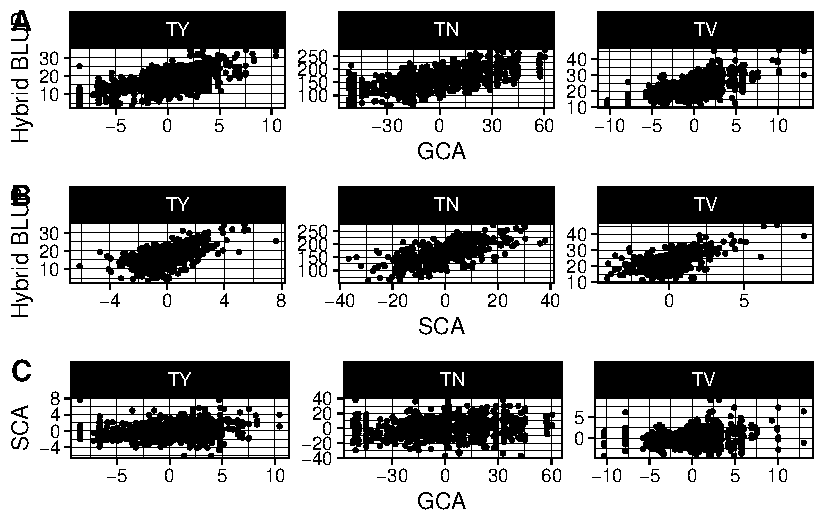
\includegraphics[keepaspectratio]{figs_02/bv-sca-performance-1.pdf}}

}

\caption{Scatterplots for each tuber trait with (A) hybrid BLUP's
plotted with GCA's, (B) SCA's, and (C) GCA's on SCA's}

\end{figure}%

\begin{table}
\centering
\caption{Ratio between the sample quantiles of GCA and SCA effects for total yield (TY), tuber number (TN), and average tuber volume (TV). Included are the 0, 10th, 25th, 40th, 60th, 75th, 90th and 100th percentiles along with an average ratio of quantiles in $\overline{q}$.}
\centering
\begin{tabular}[t]{lrrrrrrrrr}
\toprule
Trait & 0\% & 10\% & 25\% & 40\% & 60\% & 75\% & 90\% & 100\% & $\overline{q}$\\
\midrule
TN & 1.4 & 2.0 & 2.4 & 2.4 & 2.5 & 2.1 & 2.2 & 1.6 & 2.1\\
TV & 2.5 & 2.0 & 1.7 & 1.6 & 1.8 & 2.1 & 1.7 & 1.4 & 1.9\\
TY & 1.4 & 2.4 & 2.0 & 2.4 & 2.3 & 2.5 & 2.0 & 1.4 & 2.0\\
\bottomrule
\end{tabular}
\end{table}




\end{document}
